\section{Introduction}
The Learning and Coding agents share concept evidence but address different educational actions. Learning supports explanation and conceptual practice. Coding checks the student's ability to express an idea as executable Python. A shared model allows their observations to interact without pretending that a good verbal answer and a correct program are the same skill.

Both agents are accessible through the common natural-language input and direct buttons. The available topic lists are starting suggestions rather than the complete set of possible requests. Students can type a topic when it is not listed. Custom coding topics require successful bounded package generation and are not guaranteed to produce a usable exercise in every case.

\section{Learning Agent Workflow}
A learning request enters the existing learning runtime with the selected concept and shared student state. The service prepares an explanation and available educational resources. The interface presents the lesson within the same study workspace, together with practice and topic controls. Optional details remain collapsed until opened.

The learning workflow is state-aware. Prior assessed performance, confidence and misconception hypotheses can influence the kind of help requested. The generated explanation is content for the student to study; it is not a completed assessment. The system does not increase mastery because a lesson was displayed, because a link was opened or because the student continued to another activity.

A study-planning service also uses recorded concept information and configured topic relationships to suggest useful work. These suggestions are inspectable recommendations. They should not be presented as a learned optimal curriculum or proof that prerequisites have been mastered.

\section{Adaptive Questions and Difficulty Control}
When the student starts practice, the backend creates or resumes a topic-specific practice session. The question-generation service receives a difficulty and misconception target selected by the existing practice policy. The language model produces content that follows this decision; it does not have unrestricted authority to choose the difficulty.

The first question uses the current cognitive state. An unassessed concept starts with an easy question. Known misconceptions can require foundational work, while an uncertain hypothesis can require verification. Later questions use the latest session attempt as well as CACM. A fully incorrect answer maintains the current difficulty and probes the observed weakness. A partially correct answer also maintains difficulty to collect stronger evidence. A correct answer may increase difficulty by at most one level, subject to the mastery guardrail.

This is the implemented within-session learning policy, not the coding policy. The two should not be described as identical. In particular, the Coding Agent's state thresholds can produce a larger difficulty change, whereas the adaptive learning session explicitly limits an upward step to one level.

\begin{table}[htbp]\centering\small
\caption{Adaptive learning decisions within an active practice session}\label{tab:learning-policy}
\begin{tabular}{P{0.37\textwidth}P{0.54\textwidth}}\toprule
Latest observation & Policy response\\\midrule
No session attempt yet & Select from current CACM; no assessed history starts easy.\\
Performance equals zero & Keep the level; target observed weaknesses.\\
Performance strictly between zero and one & Keep the level and collect more evidence.\\
Performance reaches full correctness & Increase by at most one level unless the mastery guardrail prevents it.\\
Known or uncertain misconception & Include relevant verification or remediation targets.\\\bottomrule
\end{tabular}
\end{table}

\section{Topic-Specific Practice and Recovery}
A later refinement addressed a practical interface error: changing the lesson topic could leave the previous topic's question visible. The web service now binds visible practice to the active concept and preserves separate unfinished sessions. The current question's difficulty is displayed explicitly. Returning to a topic can restore its supported unfinished session rather than attach its question to a different lesson.

Question identifiers and assessment records provide a stable connection between a submitted answer and the question that was actually asked. A repeated completed answer does not create duplicate evidence. Refresh recovery restores the question and its saved state; it is not an instruction to generate a fresh question automatically.

Figure~\ref{fig:learning-ui} shows a direct browser capture of the implemented learning workspace. The profile and content in this figure are controlled fixtures, not records from a student experiment.
\begin{figure}[htbp]\centering
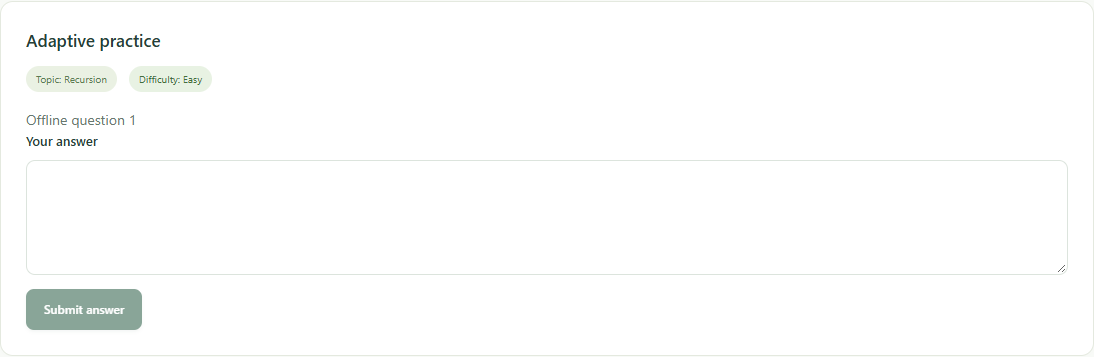
\includegraphics[width=0.98\textwidth,keepaspectratio]{learning-practice-detail.png}
\caption{Detail of topic-bound adaptive practice and an explicit difficulty label. Synthetic offline fixture.}\label{fig:learning-ui}
\end{figure}

\section{Coding Agent: Exercise Selection}
A request for practice loads a Python exercise chosen using the current concept state. The verified catalogue contains Recursion, Prime Numbers, Arrays, Strings, Python Functions and Searching Algorithms, with supported difficulty variants. For a topic outside this catalogue, the existing generator attempts to produce a structured task package and validates it before publication.

The initial coding decision is not random. If the student has no assessed attempts for the topic, or a known misconception needs remediation, the policy selects easy foundational practice. An uncertain misconception can select medium verification. Otherwise, mastery below 0.40 selects easy, mastery below 0.70 selects medium, and mastery at or above 0.70 selects hard. At high mastery, confidence affects whether the reason is verification or advanced extension.

An active cross-agent conflict has priority over these ordinary rules. The agent requests a diagnostic action rather than continuing normal progression. Table~\ref{tab:coding-policy} records the policy order, which matters because the first applicable branch wins.
\begin{table}[htbp]\centering\small
\caption{Ordered Coding Agent selection policy}\label{tab:coding-policy}
\begin{tabular}{P{0.46\textwidth}P{0.44\textwidth}}\toprule
Condition checked & Action / difficulty\\\midrule
Active cross-agent conflict & Diagnostic coding action; normal next-practice start blocked.\\
No assessed attempts or known misconception & Foundational / easy\\
Uncertain misconception hypothesis & Verification / medium\\
Mastery below 0.40 & Foundational / easy\\
Mastery at least 0.40 and below 0.70 & Guided / medium\\
Mastery at least 0.70, confidence below 0.50 & Verification / hard\\
Mastery at least 0.70, confidence at least 0.50 & Advanced / hard\\\bottomrule
\end{tabular}
\end{table}

Because CACM is shared, assessed learning history can influence the first coding exercise on that concept. A new coding interaction is not necessarily the student's first assessed encounter with the topic. At the same time, simply reading a lesson cannot justify increasing the coding level.

\section{Generated Exercise Validation}
An open-topic package includes a task title, specification, difficulty, function signature, starter code, progressive hints, supplied tests and a reference solution. Validation checks structure and supported Python behaviour, then runs the package's reference solution against its tests. The web path bounds generation to two candidate attempts.

This process reduces obvious unusable packages, but its limits are important. The model may generate both the tests and the reference solution, so they may share the same misunderstanding. Passing those tests establishes consistency with the supplied contract, not independent proof that the task specification is scientifically or pedagogically ideal. The reference solution is not included in the public exercise response shown to the student.

Only Python function-based practice is supported by this path. Unsupported language requests are not silently executed as another language. Code execution is bounded, but it is intended for trusted local use rather than hostile public submissions.

\section{Original Submission and Evaluation}
The student writes in the Monaco editor and can save a draft or request progressive hints. Submit and evaluate sends the original code to the existing submission controller and integrated workflow. Static analysis checks syntax. If the program cannot parse, the evaluator can return an objective syntax failure without asking a language model to decide whether invalid syntax is correct.

For parsable code, the runner executes the supplied behavioural tests. The returned evidence includes individual expected and actual values, errors and timeout information. The evaluator uses these observations together with model-supported feedback. The original-code assessment is the candidate for CACM integration; a later generated correction is not substituted for it.

Duplicate submission identifiers incorporate student, concept, task identity, difficulty and source code, with generated-package identity where applicable. A repeated completed submission returns the saved result without a second mastery update. A genuinely changed program can be evaluated as a new attempt.

\section{Standalone Code Review and Correction}
The application distinguishes ``give me a problem'' from ``check my existing code.'' A supplied-code request can open a persistent review editor containing the student's program and an expected-behaviour field. Deterministic syntax inspection and AI review explain supported issues and may suggest a correction.

Standalone review does not automatically execute the supplied program and does not invent tests to claim a pass. The interface labels that limitation. In assessed exercise review, a proposed correction can be checked against the loaded task's existing tests. That verification is still about the proposed correction, not about the student independently solving the exercise.

This distinction supports responsible feedback. The application can help a student understand a mistake without awarding mastery for copying an AI-written answer. If review generation fails, the original draft and completed assessment remain available for an explicit retry.

\section{Personalised Next Coding Practice}
After a completed original practice assessment, a \textit{Practise this next} card presents a recommendation. It contains the topic, difficulty, policy reason, supplied-test summary and focus derived from actual failed cases or evaluation-reported misconceptions. The recommendation reads the current shared CACM and the original submission result.

The implementation supports three ordinary outcomes. A different verified task can be loaded at the chosen level. If revision is needed and the selected task would otherwise be the same, the agent offers a targeted retry with the existing source preserved. If the student has succeeded and no different catalogue task is available at the chosen level, the system can request a new validated variant when the student explicitly starts it.

The follow-up guardrail prevents a failed submission from causing harder practice while its evaluated issues remain unresolved. The policy can move backward from medium to easy when the updated state calls for foundational work. It can also retain the same level. A single wrong answer is therefore not equivalent to an automatic one-level decrease.

Before starting, the backend recomputes the recommendation and verifies its token. Provider failure or duplicate generation leaves the original exercise and assessment in place. Matching prior behavioural contracts and matching titles are rejected as new variants, although this check cannot prove semantic novelty in general.

\begin{figure}[htbp]\centering
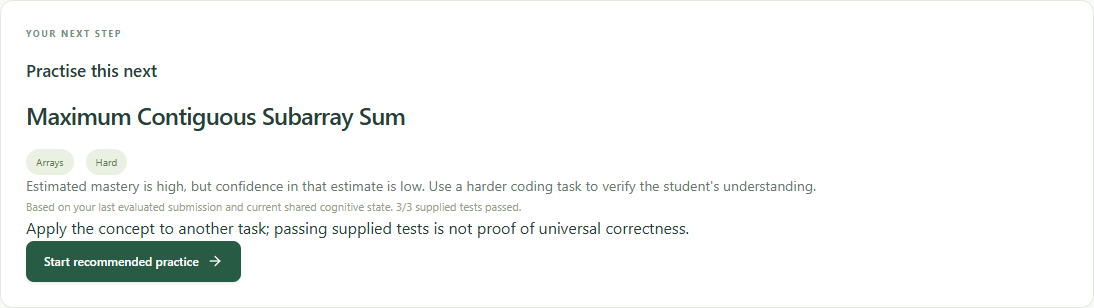
\includegraphics[width=0.98\textwidth,keepaspectratio]{coding-next-detail.png}
\caption{State-aware next-practice card after an actual fixture code assessment. Synthetic offline fixture; displayed performance is not a student-study result.}\label{fig:coding-next}
\end{figure}

\section{Worked Interaction and Interpretation}
A new profile requests an Arrays problem. With no assessed attempts, the policy begins at easy. The student submits a function, the runner checks supplied cases and the evaluator records the original result. If the code fails a boundary case, the recommendation can identify that case and retain a suitable level for revision. If a corrected original submission is accepted later, the next recommendation uses the updated state.

This example illustrates the agentic loop: observation changes the next action. It does not guarantee that the next problem is always harder, always newly generated or always on a different concept. Current coding recommendations stay within the assessed topic, and a targeted retry intentionally reuses the task when that is the supported response.
